% !TEX root = ./amsa_main.tex
\section{Composite Coordinate Friendly Operators}\label{sec:comp-cuf}
The composition of two or more operators arises in the algorithms for problems with composite functions, as well as the algorithms that are derived from operator splitting methods. To update the variable from $x^k$ to $x^{k+1}$, two or more operators are applied, and therefore the structures of all the operators together determine whether the update is CF. This is where CF structures become less trivial and more interesting. This section studies composite CF operators. The exposition leads to the recovery of existing algorithms, as well as powerful new algorithms.

\cut{Operator splitting algorithms decompose awkward combinations of operators into simpler subproblems. They give rise to a lot of efficient algorithms. \rev{Aside from the widely used ADMM and the primal-dual algorithms \cite{chambolle2011first}\cite{condat2013primal}\cite{vu2013splitting}, the forward-backward splitting, the forward-backward-forward splitting, the Douglas-Rachford splitting, the forward-Douglas-Rachford splitting also find numerous applications \cite{daubechies2003iterative}\cite{combettes2005signal}\cite{o2014primal}\cite{briceno2015FDRS} in machine learning, signal processing and imaging. Morover, the development of operator splitting schemes can produce more powerful algorithms \cite{davis2015three}. Combining operator splitting and coordinate updating will give us algorithms enjoying benefits from both sides. However, naively applying coordinate update to existing algorithms may results in divergence or wrong answers.
\begin{example}[three block ADMM]
The problem:
\begin{equation}
\begin{array}{l}
\underset{x,y,z\in\RR^m}{\textnormal{minimize  }} ~f(x)+g(y)+h(z)\\
\textnormal{subject to } Ax+Bx+Cz=b,
\end{array}\label{3block}
\end{equation}
can be solved by the following ADMM iterations:
\begin{equation}
\left\{
\begin{array}{ll}
x^{k+1}&=\argmin_x f(x)+\frac{\eta}{2}\|Ax+By^k+Cz^k+\frac{s^k}{\eta}-b\|^2,\\
\begin{pmatrix}
y^{k+1}\\
z^{k+1}
\end{pmatrix}&=\argmin_{(y,z)^\top }g(y)+h(z)+\frac{\eta}{2}\|Ax^{k+1}+By+Cz+\frac{s^k}{\eta}-b\|^2,\\
s^{k+1}&=s^k+\eta(Ax^{k+1}+By^{k+1}+Cz^{k+1}-b).
\end{array}\right.
\end{equation}
However, if we apply sequential update to the $(y,z)$ subproblem, we will have the following iterative scheme:
\begin{equation}
\left\{
\begin{array}{l}
x^{k+1}=\argmin_x f(x)+\frac{\eta}{2}\|Ax+By^k+Cz^k+\frac{s^k}{\eta}-b\|^2,\\
y^{k+1}=\argmin_y g(y)+\frac{\eta}{2}\|Ax^{k+1}+By+Cz^k+\frac{s^k}{\eta}-b\|^2,\\
z^{k+1}=\argmin_z h(z)+\frac{\eta}{2}\|Ax^{k+1}+By^{k+1}+Cz+\frac{s^k}{\eta}-b\|^2,\\
s^{k+1}=s^k+\eta(Ax^{k+1}+By^{k+1}+Cz^{k+1}-b).
\end{array}\right.
\end{equation}
It is the direct extension of ADMM to three block, which is proved to be divergent in \citep{chen2014direct}
\end{example}}
This motivates us to study the mechanism to develop coordinate update algorithms based on operator splitting. In order to do this, we study when the combinations of operators is CF in  In \S\ref{sc:comb}. Then, in \S\ref{sec:splitting} review several operator splitting schemes and provide examples. \rev{We point out here that the coordinate update methods we propose, based on operator splitting schemes, all have convergence guarantee, at least for async-parallel (thus also stochastic) update \cite{Peng_2015_AROCK}}


There are many popular operator-splitting based algorithms, e.g., proximal gradient method, ADM, and primal-dual method, which reduce the original problem to simpler subproblems, each corresponding to a part of the objective or constraints. Coordinate updates can be combined with operator splitting to further simplify their subproblems and even offer better parallelism. Most operator splitting algorithms are sequential compositions of two or more operators. This section studies when their compositions are CF operators.

}

\subsection{Combinations of Operators}\label{sc:comb}
We start by an example with numerous applications. It is a generalization of Example~\ref{ex:qhloss}.
\begin{example}[scalar map pre-composing affine function]\label{exp:log-grad} Let $a_j\in \RR^m, b_j\in \RR$, and $\phi_j:\RR\to \RR$ be differentiable functions, $j \in [p]$. Let $$f(x)=\sum_{j=1}^p \phi_j(a_j^\top x +b_j).$$ Assume that evaluating $\phi'_j$ costs $O(1)$ for all $j$. Then, $\nabla f$ is CF. Indeed, let $$\cT_1 y:=A^\top y,\quad \cT_2 y := \Diag(\phi_1'(y_1),\ldots,\phi_p'(y_p)), \quad \cT_3 x := Ax+b,$$ 
where $A=[a_1^\top; a_2^\top; \ldots,a_p^\top]\in \RR^{p\times m}$ and $b=[b_1;b_2;\ldots;b_p]\in\RR^{p\times 1}$. Then $\nabla f(x)= \cT_1\circ\cT_2\circ\cT_3 x$. For any $x$ and $i\in\{1,\ldots,m\}$, let $x^+_i=\nabla_i f(x)$ and $x^+_j=x_j,\forall j\neq i$, and let $\cM(x)=\cT_3 x$. We can first compute $\cT_2\circ\cT_3 x$ from $\cT_3 x$ for $O(p)$ operations, then compute $\nabla_i f(x)$ and thus $x^+$ from $\{x, \cT_2\circ\cT_3 x\}$ for $O(p)$ operations, and finally update the maintained $\cT_3 x$ to $\cT_3 x^+$ from $\{x, x^+,\cT_3 x\}$ for another $O(p)$ operations. Formally,
\begin{align*}
&\nops{\{x,\cT_3 x\}}{\{x^+, \cT_3x^+\}}\cr
=& \nops{\cT_3x}{\cT_2\circ\cT_3 x}+\nops {\{x,\cT_2\circ\cT_3 x\}}{x^+}+\nops{\{x,\cT_3 x, x^+\}}{\{\cT_3x^+\}}\cr
=& O(p) + O(p) +O(p)=O(p).\nonumber
\end{align*}
Since $\nops{x}{\nabla f(x)}=O(pm)$, therefore
$\nabla f= \cT_1\circ\cT_2\circ\cT_3$ is CF. 

If $p=m$, $\cT_1,\cT_2,\cT_3$ all map from $\RR^m$ to $\RR^m$. Then, it is easy to check that $\cT_1$ is Type-I CF, $\cT_2$ is separable, and $\cT_3$ is Type-II CF. The last one is crucial since not maintaining $\cT_3 x$ would disqualify $\cT$ from CF. Indeed, to obtain $(\cT x)_i$, we must multiple $A_i^\top$ to all the entries of $\cT_2\circ\cT_3 x$, which in turn needs all the entries of $\cT_3 x$, computing which from scratch costs $O(pm)$.

There are general rules to preserve Type-I and Type-II CF. For example, $\cT_1\circ \cT_2$ is still Type-I CF, and $\cT_2\circ\cT_3$ is still CF but there are counter examples where  $\cT_2\circ\cT_3$  can be neither Type-I nor Type-II CF. Such properties are important for developing efficient coordinate update algorithms for complicated problems; we will fomarlize them in the following.
\end{example}

The operators $\cT_2$ and $\cT_3$ in the above example are prototypes of \emph{cheap} and \emph{easy-to-maintain} operators from $\HH$ to $\GG$ that arise in operator compositions.
\begin{definition}[cheap operator] For a composite operator $\cT=\cT_1 \circ\cdots \circ \cT_p$, an operator $\cT_i:\HH\to\GG$ is cheap if $\nops{x}{\cT_i x}$ is less than or equal to the number of remaining coordinate-update operations, in order of magnitude.
\end{definition}

\begin{definition}[easy-to-maintain operator]
%If $\cT$ maps from $\HH$ to a different space $\GG$ and it satisfies \eqref{op-cuf2}, we call it 
For a composite operator $\cT=\cT_1 \circ\cdots \circ \cT_p$, an operator $\cT_j:\HH\to\GG$ is \emph{easy-to-maintain}, if for any $x,i,\delta_i,x^+$ satisfying \eqref{singleupdate}, $\nops{\{ x,\cT_j x, x^+\}}{\cT_j x^+}$ is less than or equal to the number of remaining coordinate-update operations, in order of magnitude, \emph{or} belongs to $O(\frac{1}{\dim \GG}\nops{x^+}{\cT x^+})$.  
\end{definition}
\cut{\begin{example}[projection to the Euclidean ball]\label{ex:projball}
Let $B_2=\{x\in\RR^m:\|x\|_2\leq r\}$ and $$\cT x:=\prj_{B_2}(x).$$ By definition, %$\cT(x)=\argmin_y \{\|y-x\|_2:\|y\|_2\le r\}$
%\begin{equation}
$\cT(x) =\xi x,~\mbox{where}~\xi=\min\left\{1,\frac{r}{\|x\|_2}\right\}.$
%\end{equation}
Since $\cT x$ depends on all the entries of $x$,  $\cT$ is non-separable.

Nonetheless, the norm map $\cT':x\mapsto \|x\|_2$ is easy-to-maintain. Indeed, given $x$, we can maintain $\cT'(x)=\|x\|_2$. If $x_i$ is updated,  letting $e_i$ be the $i$th standard basis and writing $\bar{x}=x+\eta e_i$, it follows $\|\bar{x}\|_2=\sqrt{\|x\|_2^2+2\eta x_i+\eta^2}$. Therefore,   $\nops{\{x,\|x\|_2,\eta\}}{\|\bar{x}\|_2}=O(1)$ while $\nops{\bar{x}}{\|\bar{x}\|_2}=O(m)$.

\end{example}
}

\cut{\begin{example}[Projection to Euclidean ball]
Let $\cT \, x = \Proj_{\|x\|_2 \leq r} (x)$, $\tilde x  = x + \sum_{i \in \II} \eta_i e_i$
\begin{equation}
\cT \, (\tilde x) =
\left\{
\begin{array}{ll}
\tilde x &\text{ if } \|\tilde x\| \leq r \\
\frac{r}{\|\tilde x\|} \tilde x &\text{ if } \|\tilde x\| > r,
\end{array}
\right.
\end{equation}
Note that $\|\tilde x\|^2 = \|x\|^2 + 2 \sum_{i \in \II} \langle x_i + \eta_i, \eta_i \rangle$. If $ \|\tilde x\| \leq r$, then $\cT$ is easy to update if and only if $ \|\tilde x\| \leq r$.
\end{example}}


The splitting schemes in \S\ref{sec:splitting} below will be based on $\cT_1+\cT_2$ or $\cT_1\circ\cT_2$. If $\cT_1$ and $\cT_2$ are both CF, $\cT_1+\cT_2$ must be CF while $\cT_1\circ\cT_2$ is not necessarily so. This subsection discusses how $\cT_1\circ\cT_2$ inherits the properties from $\cT_1$ and $\cT_2$, and we summarize the results in Tables \ref{table:comp1-op} and \ref{table:comp-op}.

The combination \cut{$\cT_1+\cT_2$ and }$\cT_1\circ \cT_2$ generally inherits the \emph{weaker} property from $\cT_1$ and $\cT_2$. %If one of them is separable and the other nearly-separable, then $\cT_1\circ \cT_2$ is nearly-separable. % since the composition depends on more than one coordinate of $x$.

The separable ($\cC_1$) property  is  preserved by composition. If $\cT_1,\ldots,\cT_n$ are separable, then $\cT_1\circ\cdots\circ \cT_n$ is separable.  However, combining  nearly-separable ($\cC_2$) operators  may not yield a nearly-separable operator since\cut{ Even if  $\cT_1,\ldots,\cT_n\in\cC_2$ and each $(\cT_jx)_i$ depends on $c>1$ coordinates of $x$, the composition $(\cT_1\circ\cdots\circ \cT_n x)_i$ can depend on the much more $\min\{c^n,m\}$ components of $x$, as} composition introduces cross dependence on the input entries. Therefore, composition of nearly-separable operators can be either nearly-separable or non-separable.

%\begin{center}\begin{tabular}{|c|c|c|}\hline
%$\cT_1$ & $\cT_2$ & $\cT_1+\cT_2$\\\hline
%$\cC_1$ & $\cC_1$/$\cC_2$/$\cC_3$ & $\cC_1$/$\cC_2$/$\cC_3$\\\hline
%$\cC_2$ & $\cC_2$ & $\cC_2$ or $\cC_3$\\\hline
%$\cC_2$/$\cC_3$ & $\cC_3$ & $\cC_3$\\\hline
%\end{tabular}\end{center}
%\begin{center}\begin{tabular}{c|l|l|l|l}
%Case & $\cT_1\in$ & $\cT_2\in$ & $~(\cT_1+\cT_2) \in~$ & $~(\cT_1\circ\cT_2)\in ~$\\\hline\hline
%1 & $\cC_1$ (separable) & $\cC_1$, $\cC_2$, $\cC_3$ & \multicolumn{2}{|l}{$\cC_1$, $\cC_2$, $\cC_3$, respectively}\\\hline
%2 & $\cC_2$ (nearly-sep.)& $\cC_1$, $\cC_3$ & \multicolumn{2}{|l}{$\cC_2$, $\cC_3$, respectively}\\\hline
%3 & $\cC_2$ & $\cC_2$ & \multicolumn{2}{|l}{$\cC_2$ or $\cC_3$, case by case}\\\hline
%4 & $\cC_3$ (non-sep.) & $\cC_1$, $\cC_2$, $\cC_3$ & \multicolumn{2}{|l}{$\cC_3$}\\\hline
%5 & $\cC_1$, $\cC_2$ & $\cF$ & \multicolumn{2}{|l}{$\cF$}\\\hline
%6 & $\cF$ & $\cC_1$, $\cC_2$ & $\cF$ & $\cE$\\\hline
%7 & $\cF$ & $\cF$ & $\cF$ & case by case\\\hline
%\end{tabular}\end{center}

\begin{table}
\begin{center}
\begin{tabular}{c|l|l|l}
\hline
Case & $\cT_1\in$ & $\cT_2\in$ & $~(\cT_1\circ\cT_2)\in ~$\\\hline\hline
1 & $\cC_1$ (separable) & $\cC_1$, $\cC_2$, $\cC_3$ & $\cC_1$, $\cC_2$, $\cC_3$, respectively \\\hline
2 & $\cC_2$ (nearly-sep.)& $\cC_1$, $\cC_3$ & $\cC_2$, $\cC_3$, resp. \\\hline
3 & $\cC_2$ & $\cC_2$ & $\cC_2$ or $\cC_3$, case by case \\\hline
4 & $\cC_3$ (non-sep.) & $\cC_1\cup\cC_2\cup\cC_3$ & $\cC_3$ \\\hline
\end{tabular}\end{center}
\caption{$\cT_1\circ\cT_2$ inherits the weaker separability properties from those of $\cT_1$ and $\cT_2$.}\label{table:comp1-op}\end{table}


\begin{table}
\begin{center}
\begin{tabular}{c|l|l|l|l}
\hline
Case & $\cT_1\in$ & $\cT_2\in$ & $~(\cT_1\circ\cT_2)\in ~$& Example\\\hline\hline
%1 & $\cC_1$ (separable) & $\cC_1$, $\cC_2$, $\cC_3$ & $\cC_1$, $\cC_2$, $\cC_3$, respectively & $D_1D_2$, $DA_s$, $DA_d$, resp.\\\hline
%2 & $\cC_2$ (nearly-sep.)& $\cC_1$, $\cC_3$ & $\cC_2$, $\cC_3$, resp. & $A_sD$, $A_sA_d$, resp.\\\hline
%3 & $\cC_2$ & $\cC_2$ & $\cC_2$ or $\cC_3$, case by case & $T_1T_2$\\\hline
%4 & $\cC_3$ (non-sep.) & $\cC_1\cup\cC_2\cup\cC_3$ & $\cC_3$ & $A_dB$\\\hline

%5 & $\cC_1$ & $\cF$, $\cF_1$\cut{, $\cF_2$} & $\cF$, $\cF_1$\cut{, $\cF_2$}, resp. & Example \ref{alg:prox-grad}\\\hline
%6 & $\cF$, $\cF_2$ \cut{, $\cF_1$, $\cF_2$} & $\cC_1$ & $\cF$, $\cF_2$\cut{, $\cF_1$, $\cF_2$, resp.}& Example \ref{exp:log-grad}\\\hline
%7 & $\cC_2$ & $\cF$, $\cF_1$ & $\cF$, $\cF_1$, resp. & Example \ref{exp:sp-dens} \\\hline
5 & $\cC_1\cup\cC_2$ & $\cF$, $\cF_1$\cut{, $\cF_2$} & $\cF$, $\cF_1$\cut{, $\cF_2$}, resp. & Examples~\ref{exp:sp-dens} and~\ref{alg:prox-grad}\\\hline
6 & $\cF$, $\cF_2$ \cut{, $\cF_1$, $\cF_2$} & $\cC_1$ & $\cF$, $\cF_2$\cut{, $\cF_1$, $\cF_2$}, resp.& Example \ref{exp:log-grad}\\\hline
7 & $\cF_1$ & $\cF_2$& $\cF$ &Example \ref{den-den}\\\hline
8 & cheap & $\cF_2$ & $\cF$ & Example \ref{alg:prox-grad}\\\hline
9 & $\cF_1$ & cheap& $\cF_1$ &Examples~\ref{exp:log-grad} and~\ref{alg:prox-grad}\\\hline
\end{tabular}\end{center}
\caption{Summary of how $\cT_1\circ\cT_2$ inherits CF properties from those of $\cT_1$ and $\cT_2$.}\label{table:comp-op}\end{table}
%\smallskip
%However, if  $\cT_1,\ldots,\cT_n\in\cC_2$, we may not have  $\cT_1\circ\cdots\circ \cT_n\in\cC_2$ since $(\cT_1\circ\cdots\circ \cT_n x)_i$ may depend on $\min\{c^n,m\}$ components of $x$ and thus the composite operator generally belongs to $\cC_3$ instead. Therefore, we include ``(or $\cC_3$)'' in the table.
%When we consider whether an operator is coordinate update friendly or not, we only have to consider the more complicate operator if the computation
%\end{remark}

Next, we discuss how $\cT_1\circ \cT_2$ inherits the CF properties from $\cT_1$ and $\cT_2$, and the results are summarized in Table \ref{table:comp-op}. For simplicity, we only use matrix-vector multiplication as examples in this subsection; more interesting examples will be given later.%where at least one operator in the composition is non-separable. 
\begin{itemize}

\item If $\cT_1$ is separable or nearly-separable ($\cC_1\cup\cC_2$), then as long as $\cT_2$ is CF ($\cF$), $\cT_1\circ\cT_2$ remains CF. In addition, if $\cT_2$ is Type-I CF ($\cF_1$), so is $\cT_1\circ\cT_2$; see Example~\ref{exp:sp-dens}. 
\begin{example}\label{exp:sp-dens}
Let $A\in\RR^{m\times m}$ be \emph{sparse} and $B\in\RR^{m\times m}$ \emph{dense}. Then $\cT_1 x=Ax$ is nearly-separable and $\cT_2 x=Bx$ is Type-I CF.  For any $i$, let $\II_i$ index the set of nonzeros on the $i$th row of $A$. We first compute\footnote{For this example, one can of course pre-compute $AB$ and claim that $(\cT_1\circ\cT_2)$ is Type-I CF. Our arguments keep $A$ and $B$ separate and only use the nearly-separability of $\cT_1$ and Type-I CF of $\cT_2$, so our result holds for any such composition even when $\cT_1$ and $\cT_2$ are nonlinear.} $(Bx)_{\II_i}$ that costs $O(|\II_i|m)$ and then $a_{i,\II_i} (Bx)_{\II_i}$ that costs $O(|\II_i|)$, where $a_{i,\II_i}$ is formed by the nonzeros entries on the $i$th row of $A$. Assume $O(|\II_i|)=O(1),\,\forall i$. We have, from the above discussion, that $\nops{x}{(\cT_1\circ\cT_2 x)_i}=O(m)$,
while $\nops{x}{\cT_1\circ\cT_2 x}=O(m^2)$. Hence, $\cT_1\circ\cT_2$ is Type-I CF.
\end{example}


\item Assume that $\cT_2$ is separable ($\cC_1$). It is easy to see that if $\cT_1$ is CF ($\cF$)\cut{ ($\cF, \cF_1, \cF_2$)}, then $\cT_1\circ \cT_2$ remains CF\cut{ ($\cF, \cF_1, \cF_2$, respectively)}. In addition if $\cT_1$ is Type-II CF ($\cF_2$), so is $\cT_1\circ\cT_2$; see Examples \ref{exp:log-grad}.\cut{ and \ref{alg:prox-grad}.} %The results are summarized in Cases 5 and 6 of Table \ref{table:comp-op}.

Note that if $\cT_2$ is nearly-separable, in general we do not have CF properties for $\cT_1\circ\cT_2$. This is because $\cT_2 x$ and $\cT_2 x^+$ can be totally different (so updating $\cT_2 x$ is expensive) even if $x$ and $x^+$ differ only at one coordinate; see the example in footnote~\ref{note1}. %We have three sub-cases: Sub-case (i): If $\cT_2$ is easy-to-update, then  $\cT$ is CF\cut{easy-to-update provided that we maintain $\cT_2 x$}. Sub-case (ii): If $\cT_2$ is CF, then so is $\cT$. \cut{We say that $\cT_2$ is \emph{easy-to-compute} if $\nops{x}{\cT_2 x}\le \nops{\cT_2x}{(\cT_1(\cT_2 x))_i}$ for all $i$. Clearly, if $\cT_2$ is easy-to-compute, then $\cT=\cT_1\circ \cT_2$ is CF. Sub-case (iii): If $\cT_2x = Ax+b$, then $\cT=\cT_1\circ \cT_2$ is CF since, for each $i$, there exists $\cT_{1,i}$ such that  $(\cT x)_i=\cT_{1,i}(\cT_2 x)_i=\cT_{1,i}(a_i^\top x+b_i)$.}


\item Assume that $\cT_1$ is Type-I CF ($\cF_1$). Then if $\cT_2$ is Type-II CF ($\cF_2$), $\cT_1\circ\cT_2$ must be CF ($\cF$); see the next example.
\begin{example}\label{den-den}
Let $A,B\in\RR^{m\times m}$ be dense. Then $\cT_1 x=Ax$ is Type-I CF and $\cT_2 x=Bx$ Type-II CF (by maintaining $Bx$; see {Example \ref{ex:lsq2}}). For any $x$ and $i$, let $x^+$ satisfy \eqref{singleupdate}. Maintaining $\cT_2 x$, we can compute $\cT_2 x^+$ for $O(m)$ operations and then $(\cT_1\circ\cT_2 x^+)_j$ for $O(m)$ operations for any $j$. On the other hand, computing $\cT_1\circ\cT_2 x^+$ without maintaining $\cT_2 x$ costs $O(m^2)$. 
\end{example}

%\item Consider the case where $\cT_1$ is non-separable.  There are two sub-cases. (a): If $\cT_1$ is CF, then if $\cT_2$ is separable and we maintain $\cT_2 x$, $\cT_1\circ \cT_2$ remains CF. Indeed, suppose that $x$ changes to $\tilde x = x+\eta e_i$. Then, only one coordinate of $\cT_2 x$ becomes different, allowing a quick update to $\cT \tilde x=\cT_1(\cT_2 \tilde x)$. (b): If $\cT_1$ is Type-I CF, then \emph{only if} $\cT_2$ is easy-to-compute, does $\cT=\cT_1\circ \cT_2$ remain CF; see Cases 6 and 7 in Table \ref{table:comp-op}. \cut{If $\cT_1 y = Ay+b$ (which is CF) where $\cA\in\RR^{m\times m}$, then \emph{only if} $\cT_2$ is  easy-to-update or is easy-to-compute (specifically, $\nops{x}{T_2x}\le O(m)$), is $\cT=\cT_1\circ \cT_2$ remain CF. Indeed, since $(\cT x)_i = a_i^\top (\cT_2 x)+b_i$, we must be able to update $\cT_2 x$ or compute it quickly.}

\item Assume that one of $\cT_1$ and $\cT_2$ is cheap\cut{\footnote{By ``cheap'', we mean their computational complexity differ at least one order. For example, if computing $\cT_1 x$ costs $O(m)$ and $\cT_2 x$ costs $O(m^2)$, then $\cT_1$ is cheap.} compared to the other one}. If $\cT_2$ is cheap, then as long as $\cT_1$ is Type-I CF ($\cF_1$), $\cT_1\circ \cT_2$ is Type-I CF. If $\cT_1$ is cheap, then as long as $\cT_2$ is Type-II CF ($\cF_2$), $\cT_1\circ \cT_2$ is CF ($\cF$); see Example~\ref{alg:prox-grad}.
\end{itemize}

We will see more examples of the above cases in the rest of the paper.
\cut{
\rev{\subsection{Demonstration with Logistic Regression}
In this subsection, we compare the efficiency of three coordinate update schemes (cyclic, cyclic permutation, and random) with the full gradient descent method for solving the regularized logistic regression problem 
\begin{equation}\label{eqn:l2_log}
\Min_{x} \frac{\lambda}{2} \|x\|_2^2 + \sum_{i = 1}^p \log\left(1 + \exp(- b_i \cdot a_i^\top x)\right).
\end{equation}
The goal of this experiment is to show the efficiency of the coordinate update methods for composition operators. We solve \eqref{eqn:l2_log} with the following gradient descent method
\begin{equation}\label{eqn:gd_for_log_loss}
x^{k+1} = x^k - \eta_k \left(\lambda  x^k + \sum_{i = 1}^p \frac{-b_i}{1 + \exp{(b_i \cdot a_i^\top  x^k)}} a_i\right),
\end{equation}
where $\eta_k$ is the step size. The update \eqref{eqn:gd_for_log_loss} can be treated as a combination of the four operators ($\cI, A, A^\top, \cT$), i.e., 
\begin{equation}\label{eqn:log-reg-update}
x^{k + 1} = (1 - \lambda \eta_k) \cI x^k + \eta_k A^\top \circ \cT \circ A x^k,
\end{equation}
where $\cT(y) = (\frac{b_1}{1 + \exp(b_1 \cdot y_1)}, ..., \frac{b_p}{1 + \exp(b_p \cdot y_p)})^\top$ and $A = (a_1,  ..., a_p)^\top \in \RR^{p \times m}$. As explained in Example \ref{exp:log-grad}, the update \eqref{eqn:log-reg-update} is CF if $Ax^k$ is maintained. It is worth mentioning that greedy coordinate update with Gauss-Southwell rule is not an efficient choice for solving \eqref{eqn:l2_log}, since the complexity of computing the scores is $O(mp)$ even though $Ax^k$ is maintained. We test \eqref{eqn:log-reg-update} with $A$ and $x$ generated with standard normal distribution, and $b = \sign (Ax)$. We set $m = p = 100$, and set $\lambda = 0$ and $\lambda = 1$ for the first and the second experiment respectively. When $\lambda = 0$, the objective is convex, but not strongly convex, so Figure \ref{fig:log_a} shows that all of the methods converge with sublinear rate. When $\lambda = 1$, the objective function is strongly convex, all methods converge with linear rate as shown in Figure \ref{fig:log_b}. In both scenarios, coordinate update methods converge faster than the full gradient descent method. 
\begin{figure}[!htbp] \centering
    \begin{subfigure}[b]{0.48\linewidth}
        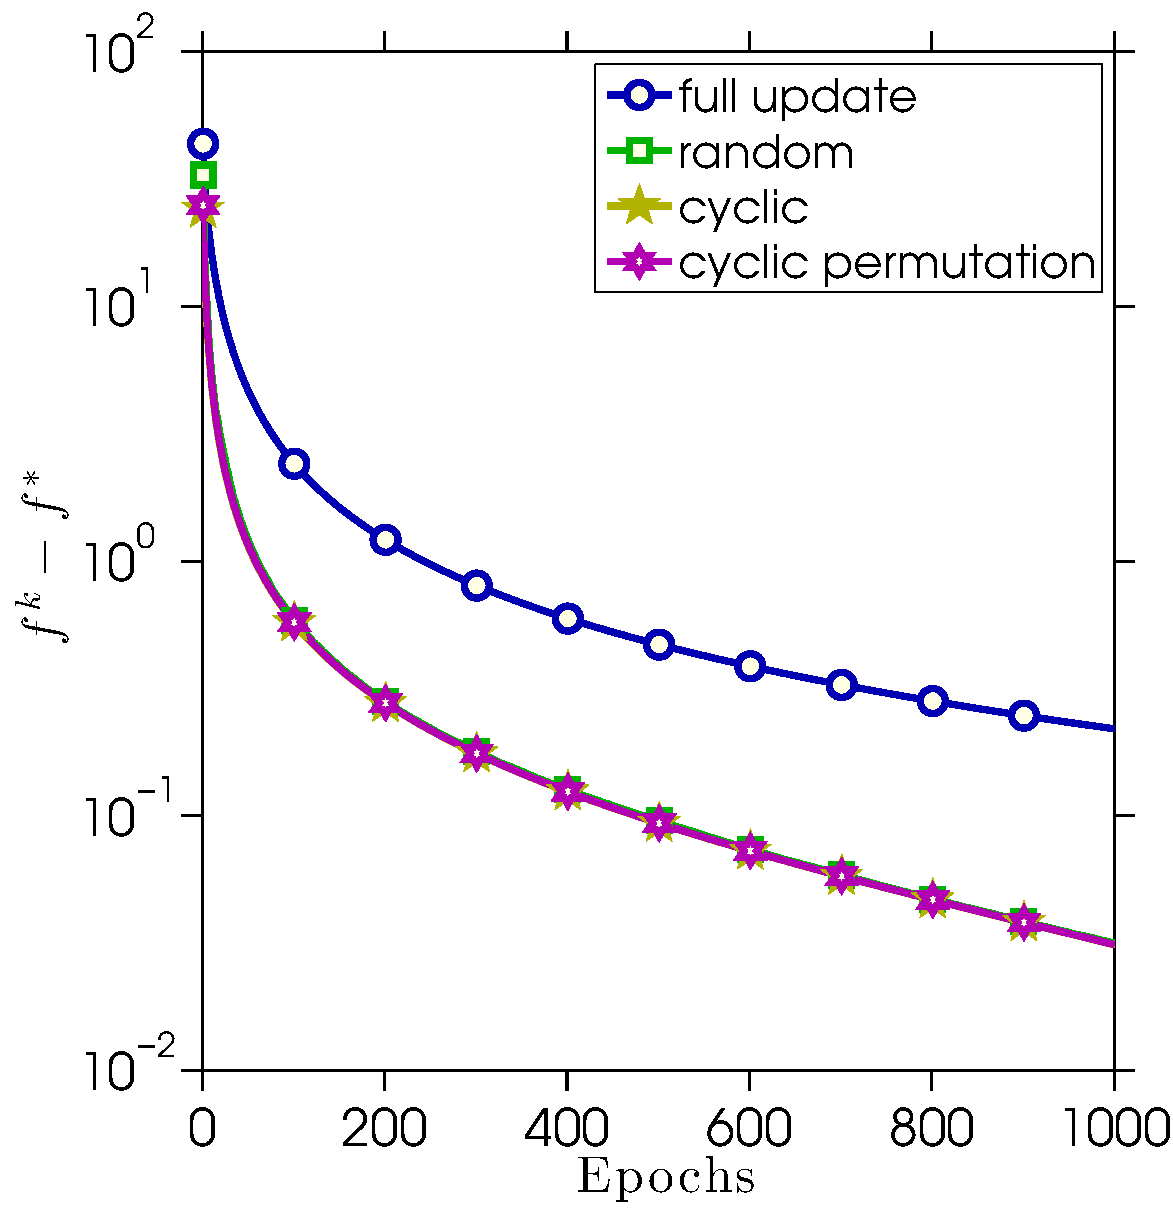
\includegraphics[width=50mm]{./figs/log_randn_matrix_lambda_0_cropped.pdf}
        \caption{$\lambda = 0$}
        \label{fig:log_a}
    \end{subfigure} %
    \quad
    \begin{subfigure}[b]{0.48\linewidth}
        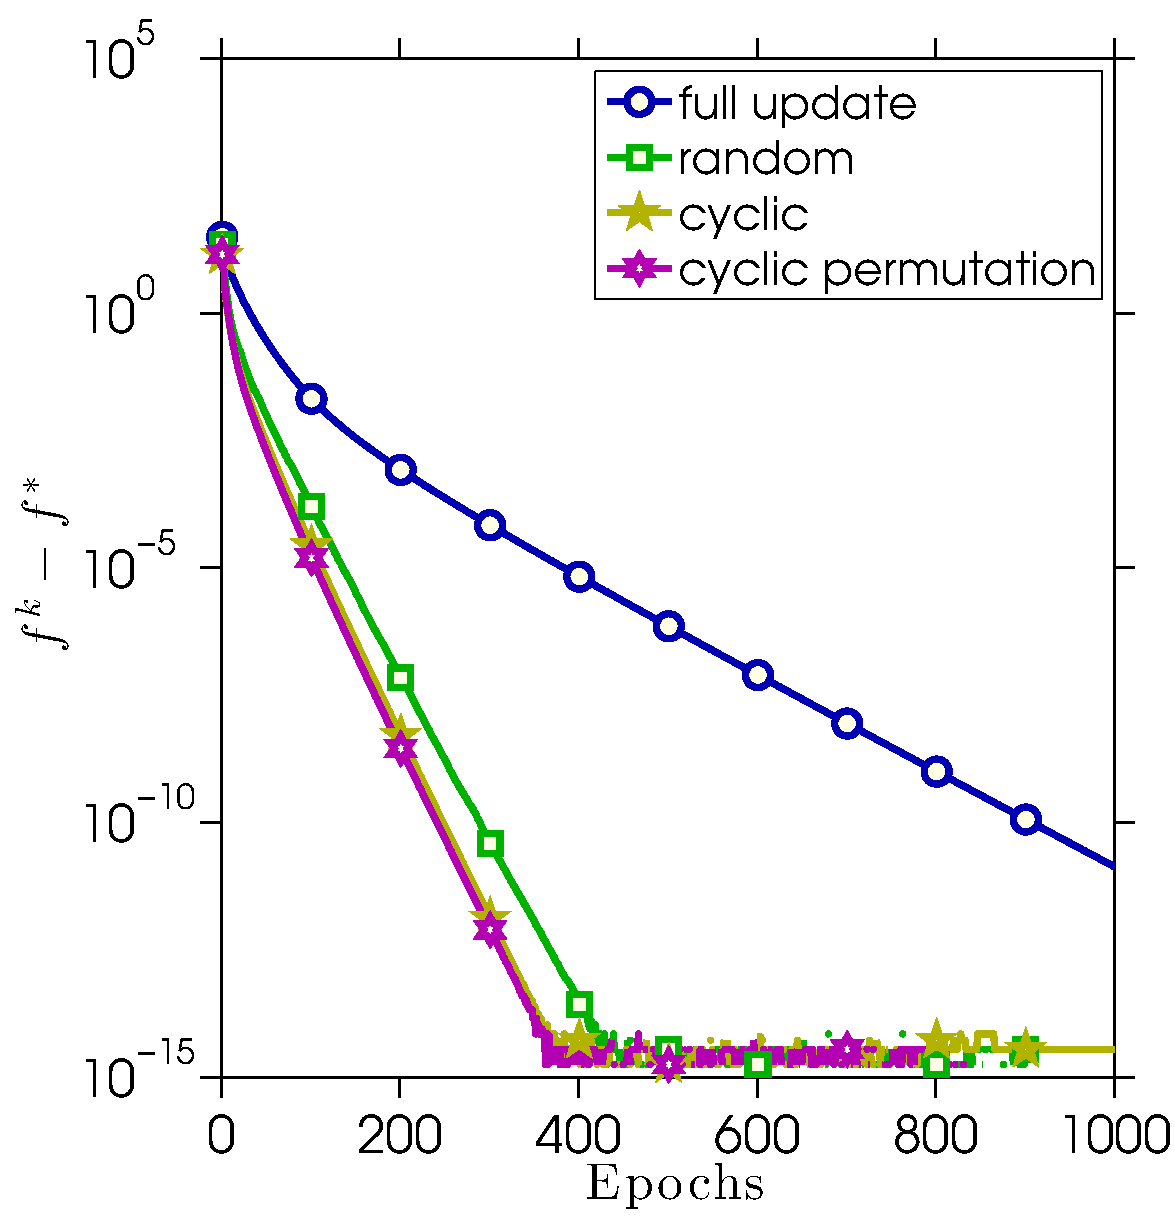
\includegraphics[width=50mm]{./figs/log_randn_matrix_lambda_1_cropped.pdf}
        \caption{$\lambda = 1$}
        \label{fig:log_b}
    \end{subfigure} %
    \caption{Compare the convergence of three different coordinate update algorithms with full gradient descent algorithm for solving logistic regression.}
    \label{fig:l2_log_results}
\end{figure}
}

\cut{If $\cT_1\in \cC_1$ and $\cT_2\in \cE$ (is easy to update), then  $\cT_1\circ \cT_2\in \cF$ is amenable for coordinate update. Specifically, we shall cache $\cT_2 x$, and when one or a few coordinates of $x$ change, we can compute $((\cT_1\circ \cT_2) x)_i$ by first refreshing $\cT_2 x$ at a low cost and then computing $((\cT_1\circ \cT_2) \tilde x)_i=(\cT_1(\cT_2x))_i$.}
}
\cut{
\begin{example}[linear composing easy-to-update] SOCP
\end{example}

\begin{example}[$\cC_1\cup \cC_2$ composing easy-to-update]
 Prox-linear / forward-backward
\end{example}
}
%\begin{example}[$\cC_1\cup \cC_2$ composing linear composing easy-to-update]
%\end{example}



\cut{
In this section, we consider operators which can be written as a composition of several simpler operators. We will discuss when the composite operators will be BC-friendly.

Assume that operator $\cT$ is a composition of two operators, i.e.,
\begin{equation}
\cT = \cT_1 \circ \cT_2.
\end{equation}
We consider the following three main cases, where \uline{BC-friendly of individual operators induces BC-friendly} of composite operator.

\begin{itemize}
\item If $\cT_1$ is with property $\cC_1$, $\cT_1\circ \cT_2$ has the same property as $\cT_2$, i.e., if $\cT_2$ is with property $\cC_1$ (or $\cC_2$, $\cC_3$, $\cB_1$, $\cB_2$, $\cB_3$), then $\cT_1\circ\cT_2$ is with property $\cC_1$ (or $\cC_2$, $\cC_3$, $\cB_1$, $\cB_2$, $\cB_3$, respectively),
\item If $\cT_1$ is with property $\cC_2$, and $\cT_2$ is with property $\cC_1$, then $\cT_1\circ\cT_2$ is with property $\cC_2$.
\item If $\cT_1$ is with property $\cC_2$, and $\cT_2$ is with property $\cC_2$, then $\cT_1\circ\cT_2$ is with property $\cC_2$.
\item If $\cT_1$ is with property $\cC_2$, and $\cT_2$ is with property $\cC_3$, then $\cT_1\circ\cT_2$ is with property $\cC_3$.
\item If $\cT_1$ is with property $\cC_2$, and $\cT_2$ is with property $\cB_1$, then $\cT_1\circ\cT_2$ is with property $\cB_1$?
\item $\cdots$
\end{itemize}

Case 1. If $\cT_1=\cT_{1,1}\times\cdots\times \cT_{1,m}$ is block-separable, then
$$ \cS_i \circ (\cT_1 \circ \cT_2) = \cT_{1,i}\circ (\cS_i \circ \cT_2).$$
If $\cT_2$ is BC-friendly, then the composite map $\cT$ is also BC-friendly.

Case 2.  If $\cT_1$ is  sparse supported, then $\exists\, \II_{i}$ such that $$(\cS_i\circ \cT_1)x = (\cT_1x)_i = \cT_{1,i}(\{x_j\}_{j\in \II_i}),$$
where $|I_i|$ is small, and thus
$$ \cS_i \circ (\cT_1 \circ \cT_2) = \cT_{1,i}(\{\cS_j \circ \cT_2\}_{just}).$$
In this case, if $\cT_2$ is BC friendly, then the composite map $\cT$ is also BC-friendly.

Case 3.  If $\cT_1$ is BC-friendly and $\cT_2 \, x$ is  easy-to-compute/update, then $\cS_i \circ (\cT_1 \circ \cT_2)(x) = (\cS_i \circ \cT_1)(\cT_2 \, x )$ and $\cT$ is BC-friendly.

}

% !TEX root = ./amsa_main.tex
\subsection{Operator Splitting Schemes}\label{sec:splitting}
Before we apply our discussions above to operator splitting schemes for new algorithms, we review several major operator splitting schemes and discuss their CF properties by using the results from \S\ref{sc:comb}. For basic operator concepts like monotonicity and cocoercivity, please refer to Appendix \ref{sec:op-concept}. The definitions of resolvent and reflective-resolvent operators $\cJ_{\cA}$ and $\cR_{\cA}$ are also given there, in~\eqref{def-resolvent} and~\eqref{def-ref}, respectively. \cut{The coordinate update methods we propose, based on operator splitting schemes, all have convergence guarantee, at least for async-parallel (thus also stochastic) update \cite{Peng_2015_AROCK}. However, naively extending existing convergent algorithms to coordinate update schemes may result in divergence or wrong solutions; see also Appendix  \ref{sec:op-concept} for a counterexample.}  %goes over the definitions and properties of operators that are used to build  and ensure their convergence.

Consider the following problem: given three operators $\cA,\cB,\cC$, possibly set-valued,  \begin{equation}\label{eqn:3s_problem}
\text{find } x \in \HH \qquad \text{ such that }  \qquad 0 \in \cA x + \cB x +\cC x.
\end{equation}
This is a high-level abstraction of many problems. The study began in the 1960s, and since then a large number of algorithms and applications have been introduced. We review a few general methods in this subsection.

When $\cA, \cB$ are maximally monotone (think it as the subdifferential $\partial f$ of a proper convex function $f$) and $\cC$ is $\beta$-cocoercive (think it as the gradient $\nabla f$ of a $1/\beta$-Lipschitz differentiable function $f$),  a solution can be found by the iteration \eqref{fpi} with $\cT=\TS$, introduced recently in \cite{davis2015three}, where  \cut{three operator splitting (3S) for solving \eqref{eqn:3s_problem} is defined by}
\beq\label{3s}
\TS := \cI- \cJ_{\gamma \cB}+ \cJ_{\gamma \cA}\circ(2 \cJ_{\gamma \cB}- \cI - \gamma \cC\circ \cJ_{\gamma \cB}).
\eeq \cut{It can be shown that if $\cC$ is $\beta$-cocoercive, then}Indeed, by setting  $\gamma\in(0,2\beta)$, $\cT_{3S}$ is $(\frac{2\beta}{4\beta-\gamma})$-averaged (think it as a weaker property than the Picard contraction that does not guarantee $\cT$ having a fixed point). Following the standard convergence result (cf. textbook \cite{B-C2011cvx-mon}), provided that $\cT$ has a  fixed point, the sequence from~\eqref{fpi} converges to a fixed-point $x^*$ of $\TS$. Instead of $x^*$, $\cJ_{\gamma\cB}(x^*)$ is a solution to~\eqref{eqn:3s_problem}.  \cut{, and one can choose $\gamma\in(0,2\beta)$ for convergence.}
Applying the results in \S\ref{sc:comb},  $\TS$ {is CF if } $\cJ_{\gamma \cA}$ is separable ($\cC_1$), $\cJ_{\gamma \cB}$ is \cut{easy-to-compute or }Type-II CF ($\cF_2$), and $\cC$ is Type-I CF ($\cF_1$). %Given $x$, $(\cT_{3S} x)_i = ......$

%\subsubsection{Special cases}
We give a few special cases of $\TS$ below, which have much longer history. They all converge to a fixed point $x^*$ whenever a solution exists and $\gamma$ is properly chosen. Whenever $\cB\neq 0$, {$\cJ_{\gamma \cB}(x^*)$ replaces $x^*$  as a solution to \eqref{eqn:3s_problem}.

 \textbf{Forward-Backward Splitting (FBS):} Letting $\cB=0$ yields $\cJ_{\gamma\cB}=\cI$. Then, $\TS$ reduces to FBS \cite{passty1979FBS}:
 \begin{equation}\label{eq:FBS}
 \TFBS:=\cJ_{\gamma \cA}\circ(\cI-\gamma \cC)
 \end{equation}
 for solving the problem $0\in\cA x+\cC x$.

\textbf{Backward-Forward Splitting (BFS):} Letting $\cA=0$ yields $\cJ_{\gamma\cA}=\cI$. Then, $\TS$ reduces to BFS:
  \begin{equation}\label{eq:BFS}\TBFS:=(\cI-\gamma \cC)\circ \cJ_{\gamma \cB}
  \end{equation}
for solving the problem $0\in\cB x+\cC x$. When $\cA=\cB$, $\TFBS$ and $\TBFS$ apply the same pair of operators in the opposite orders, and they solve the same problem. Iterations based on $\TBFS$ are rarely used in the literature because they  need an extra application of $\cJ_{\gamma B}$ before returning the solution, so $\TBFS$ is seemingly an unnecessary variant of $\TFBS$. However, they become  different in coordinate update algorithms; in particular, $\TBFS$ is CF (but $\TFBS$ is generally not) when $\cJ_{\gamma \cB}$ is \cut{easy-to-compute or }Type-II CF ($\cF_2$) and $\cC$ is Type-I CF ($\cF_1$). Therefore, $\TBFS$ is worth discussing alone.

\textbf{Douglas-Rachford Splitting (DRS):} Letting $\cC=0$, $\TS$ reduces to 
  \begin{equation}\label{eq:DRS}\TDRS:=\cI-\cJ_{\gamma \cB}+\cJ_{\gamma\cA}\circ(2\cJ_{\gamma \cB}-\cI)=\frac{1}{2}(\cI+\cR_{\gamma\cA}\circ \cR_{\gamma\cB})
  \end{equation}
introduced in \cite{douglas1956DRS} for solving the problem $0\in\cA x+\cB x$. A more general splitting is the  Relaxed Peaceman-Rachford Splitting (RPRS) with $\lambda\in[0,1]$:
 \begin{equation}
\cT_{\text{RPRS}} = (1 - \lambda)\, \cI + \lambda \, \cR_{\gamma \cA} \circ \cR_{\gamma \cB},
\end{equation}
which recovers $\TDRS$ by setting $\lambda=\frac{1}{2}$ and Peaceman-Rachford Splitting (PRS) \cite{peaceman1955PRS} by $\lambda=1$.

\textbf{Forward-Douglas-Rachford Splitting (FDRS):} Let $V$ be  a linear subspace, and $\cN_V$ and $\cP_V$ be the normal cone and projection operator, respectively. The FDRS~\cite{briceno2015FDRS} 
 $$\TFDRS=\cI-\cP_V+\cJ_{\gamma\cA}\circ(2\cP_V-\cI-\gamma \cP_V\circ\tilde{\cC}\circ\cP_V),$$
aims at finding a $x$ such that $0\in\cA\,x+\tilde{\cC}\,x+\cN_V\,x$. If an optimal $x$ exists, we have $x\in V$ and $\cN_Vx$ is the orthogonal complement of $V$. Therefore, the problem is equivalent to finding $x$ such that $0\in\cA\,x+\cP_V\circ\tilde{\cC}\circ\cP_V\,x+\cN_V\,x$. Thus, $\TS$ recovers $\TFDRS$ by letting $\cB=\cN_V$ and $\cC=\cP_V\circ\tilde{\cC}\circ\cP_V$.

\textbf{Forward-Backward-Forward Splitting (FBFS):} Composing $\TFBS$ with one more forward step gives $\TFBFS$ introduced in \cite{FBF_Tseng}:
\begin{align}\label{eqn:fbf}
\TFBFS = -\gamma \cC  + (\cI-\gamma \cC)\cJ_{\gamma \cA}(\cI-\gamma \cC).
\end{align} %~\cite{FBF_Tseng} for solving the problem of finding the zero in the sum of two operators, i.e.,
%\begin{equation}\label{eqn:2_problem}
%\text{find } x \in \HH \qquad \text{ such that }  \qquad 0 \in \cA\,x + \cC\,x,
%\end{equation}
%is defined in the following 
$\TFBFS$ is not  a special case of $\TS$. At the expense of one more application of $(\cI-\gamma \cC)$, $\TFBFS$ relaxes the convergence condition  of $\TFBS$ from  the cocoercivity of $\cC$ {to its monotonicity (for example, a nonzero skew symmetric matrix is monotonic but not cocoercive)}. 
From Table \ref{table:comp-op}, we know that $\TFBFS$ is CF if both $\cC$ and $\cJ_{\gamma \cA}$ are separable.

\subsubsection{Examples in Optimization}
Consider the optimization problem
\begin{equation}\label{eq:opt-example}
\Min_{x\in X}\, f(x)+g(x),
\end{equation}
where $X$ is the feasible set and $f$ and $g$ are objective functions. We present examples of operator splitting methods discussed above.

\cut{We discuss a few well-known optimization methods for solving problems in the form of \eqref{eq:opt-example} and relate them to the previous operator splitting methods.}

\begin{example}[{proximal gradient method}]\label{alg:prox-grad} Let $X=\RR^m$, $f$ be differentiable, and $g$ be proximable in \eqref{eq:opt-example}. Letting $\cA=\partial g$ and $\cC=\nabla f$ in \eqref{eq:FBS} gives $\cJ_{\gamma \cA}=\prox_{\gamma g}$ and reduces $x^{k+1}=\TFBS(x^k)$ to prox-gradient iteration: \cut{. one can apply the proximal gradient method with update}
\begin{equation}\label{eq:prox-grad}x^{k+1}=\prox_{\gamma g}(x^k-\gamma\nabla f(x^k)).
\end{equation} 
A special case of \eqref{eq:prox-grad} with $g=\iota_X$ is the projected gradient iteration:
\begin{equation}\label{eq:proj-grad}
x^{k+1}=\cP_X(x^k-\gamma \nabla f(x^k)).
\end{equation}

If $\nabla f$ is CF and $\prox_{\gamma g}$ is (nearly-)separable (e.g., $g(x)=\|x\|_1$ or the indicator function of a box constraint) or if $\nabla f$ is Type-II CF and $\prox_{\gamma g}$ is cheap (e.g., $\nabla f(x)=Ax-b$ and $g=\|x\|_2$), the FBS iteration in \eqref{eq:prox-grad} is CF. In the latter case, we can also apply the BFS iteration \eqref{eq:BFS} (i.e,  compute $\prox_ {\gamma g}$ and then the gradient update), which is also CF.

\end{example}

%\begin{example}[\textbf{Projected gradient method}]\label{alg:proj-grad} Let $f$ be differentiable and $g=0$. Then, \eqref{eq:opt-example} is a constrained smooth convex program. Let  $\cA=\cN_X$ and $\cC=\nabla f$ in \eqref{eq:FBS}. Then,\cut{ For this problem, one can apply} $x^{k+1}=\TFBS(x^k)$ recovers the projected gradient iteration:
%$$x^{k+1}=\cP_X(x^k-\gamma \nabla f(x^k)).$$
%%{Then $\cJ_{\gamma \cA}=\cP_X$, and the above update is simply $x^{k+1}=\textcolor{blue}{\TFBS}(x^k)$.}
%If $\nabla f$ is CF (e.g., $\nabla f(x)=Ax-b$) and $X$ is (nearly-)separable constraint (e.g., box constraint), the iteration is CF.
%\end{example}

\DIFdelbegin %DIFDELCMD < \begin{example}[ADMM]%%%
\DIFdelend \DIFaddbegin \begin{example}[Alternating Direction Method of Multipliers (ADMM)]\DIFaddend \label{alg:admm} Setting $X=\RR^m$ simplifies \eqref{eq:opt-example} to 
\begin{equation}\label{eq:compx-y}
\Min_{x,y}~f(x)+g(y),\quad\St~ x-y=0.
\end{equation} 
%and one can apply the alternating direction method of multiplier (ADMM) by the updates
The ADMM method iterates:
\begin{subequations}\label{eq:admmx-y}
\begin{align}
&x^{k+1}=\prox_{\gamma f}(y^k-\gamma s^k),\\%\argmin_x f(x)+\langle s^k, x-y^k\rangle + \frac{1}{2\eta}\|x-y^k\|^2,\\
&y^{k+1}=\prox_{\gamma g}(x^{k+1}+\gamma s^{k}),\\%\argmin_y g(y)+\langle s^k, x^{k+1}-y\rangle + \frac{1}{2\eta}\|x^{k+1}-y\|^2,\\
&s^{k+1}=s^k+\frac{1}{\gamma}(x^{k+1}-y^{k+1}).
\end{align}
\end{subequations}
(The iteration can be generalized to handle the constraint $Ax-By=b$.) The dual problem of \eqref{eq:compx-y} is $\min_s f^*(-s)+g^*(s)$, where $f^*$ is the convex conjugate of $f$. Letting $\cA=-\partial f^*(-\cdot)$ and $\cB=\partial g^*$ in \eqref{eq:DRS} recovers the iteration  \eqref{eq:admmx-y} through (see the derivation in Appendix \ref{sec:drs-admm})
\begin{align*}
%&s^k=\cJ_{\gamma \cB}(t^k),\\
&t^{k+1}=\TDRS(t^k)=t^k-\cJ_{\gamma \cB}(t^k)+\cJ_{\gamma\cA}\circ(2\cJ_{\gamma \cB}-\cI)(t^k).
\end{align*}  %If $\prox_{\gamma f}$ is easy-to-compute, and $\prox_{\gamma g}$ is separable, then the ADMM iteration  is CF.
From the results in \S\ref{sc:comb}, a sufficient condition for the above iteration to be CF is that $\cJ_{\gamma\cA}$ is (nearly-)separable and $\cJ_{\gamma\cB}$ being CF. 
\end{example}


%\begin{subsection}{Forward-backward splitting (FBS) and backward-forward splitting (BFS)}
%The forward-backward splitting (FBS) and the backward-forward splitting (BFS) solves the problem of finding the zero in the sum of two maximally monotone operators, i.e., it considers
%\begin{equation}\label{eqn:monotone_problem}
%\text{find } x \in \cH \qquad \text{ such that }  \qquad 0 \in \cA\,x + \cB\,x.
%\end{equation}
%The forward-backward splitting operator is the following
%\begin{equation}\label{eqn:fbs}
%\cT_{\text{FBS}} \, x= \cJ_{\gamma \cA} \circ (x - \gamma \cB \, x),
%\end{equation}
%and the backward-forward splitting operator is
%\begin{equation}\label{eqn:fbs}
%\cT_{BFS} \, x= (I - \gamma \cB) \circ \cJ_{\gamma \cA}(x),
%\end{equation}
%where $\cJ_{\gamma \cA} := (1+\gamma \, \cA)^{-1}$ is the \emph{resolvant} of $A$. It has been shown that $x$ solves \eqref{eqn:monotone_problem} if any only if $x$ is a fixed point of $\cT_{\text{FBS}}$ or $\cT_{BFS}$. As we discussed before, if $\cB$ is BC-friendly, and $J_{\gamma \cA}$ is block-separable, then $\cT_{\text{FBS}}$ is BC-friendly. However, if $J_{\gamma \cA}$ is easy-to-compute/update but not necessary block-separable, and $B$ is BC-friendly, then the $\cT_{\text{FBS}}$ is not necessary BC-friendly, but $\cT_{\text{BFS}}$ is BC-friendly. We will give some examples in Section \ref{sec:app} to illustrate the two different types of update scheme. 
%
%\end{subsection}

\cut{
\begin{subsection}{Relaxed Peaceman-Rachford splitting (RPRS)}
The relaxed Peaceman-Rachford splitting (RPRS) also targeted at solving \eqref{eqn:monotone_problem}. The RPRS is define in the following
\begin{equation}
\cT_{\text{RPRS}} = (1 - \lambda)\, \cI + \lambda \, \cR_{\gamma \cA} \circ \cR_{\gamma \cB},
\end{equation}
where $\cR_{\gamma \cA}:= 2 J_{\gamma \cA} - I$ is the reflection operator. Note that $\lambda = 1$ gives the Peaceman-Rachford splitting (PRS) operator, and $\lambda = \frac{1}{2}$ gives the Douglas-Rachford splitting (DRS) operator. 

Applying the results of composite maps, the RPRS splitting operator is CF in either of the following two cases:

Case 1. $ \cR_{\gamma A}$ is block-separable  and $\cR_{\gamma B}$ is CF.

Case 2. $ \cR_{\gamma A}$ is Type-I CF and $\cR_{\gamma B}$ is easy-to-update. 
\end{subsection}

\subsection{Forward-Backward-Forward operator splitting}
The Forward-Backward-Forward operator splitting (FBF)~\cite{FBF_Tseng} for solving the problem of finding the zero in the sum of two operators, i.e.,
\begin{equation}\label{eqn:2_problem}
\text{find } x \in \HH \qquad \text{ such that }  \qquad 0 \in \cA\,x + \cC\,x,
\end{equation}
is defined in the following 
\begin{align}\label{eqn:fbf}
\cT_{\text{FBF}} = -\gamma \cC  + (I-\gamma \cC)\cJ_{\gamma \cA}(I-\gamma \cC).
\end{align}
The advantage of FBF comparing to FBS is that the cocoercivity condition of $\cC$ is relaxed into monotonicity at the expense of additional computations.
Then, we know that $\cT_{\text{FBF}}$ is CF, if both $\cC$ and $\cJ_{\gamma \cA}$ are separable.
}

%\begin{subsection}{Three operator splitting (3S)}
%The three operator splitting method solves the problem of finding the zero in the sum of three operators ($A, B, C$), where $A, B$ are maximally monotone and $C$ is cocoercive. The three operator splitting is defined as following:
%$$\cT_{3S} = \cI- \cJ_{\gamma \cB}- \cJ_{\gamma \cA}\circ(2 \cJ_{\gamma \cB}- \cI - \gamma \cC\circ \cJ_{\gamma \cB}).$$
%Then, we know that $\cT$ is BC-friendly, if $\cJ_{\gamma \cA}$ is separable, $\cJ_{\gamma \cB}$ is easy-to-compute/update and $\cC$ is BC-friendly. 
%
%\end{subsection}



%\end{section} reduces to FBS \cite{passty1979FBS}



